\documentclass[12pt]{article}
\usepackage{etoolbox}
\usepackage{listings}
\usepackage{float}
\usepackage{graphicx}
\usepackage{color}
\usepackage[justification=centering]{caption}
\usepackage{hyperref}


\hypersetup{
	colorlinks,
	citecolor=black,
	filecolor=black,
	linkcolor=black,
	urlcolor=black
	}

\setcounter{secnumdepth}{4}
\setcounter{tocdepth}{4}

\definecolor{mygreen}{rgb}{0,0.6,0}
\definecolor{mygray}{rgb}{0.5,0.5,0.5}
\definecolor{mymauve}{rgb}{0.58,0,0.82}

\lstset{ %
	backgroundcolor=\color{white},   % choose the background color; you must add \usepackage{color} or \usepackage{xcolor}
	basicstyle=\footnotesize,        % the size of the fonts that are used for the code
	breakatwhitespace=false,         % sets if automatic breaks should only happen at whitespace
	breaklines=true,                 % sets automatic line breaking
	captionpos=b,                    % sets the caption-position to bottom
	commentstyle=\color{mygreen},    % comment style
	deletekeywords={...},            % if you want to delete keywords from the given language
	escapeinside={\%*}{*)},          % if you want to add LaTeX within your code
	extendedchars=true,              % lets you use non-ASCII characters; for 8-bits encodings only, does not work with UTF-8
	%	frame=single,                    % adds a frame around the code
	keepspaces=true,                 % keeps spaces in text, useful for keeping indentation of code (possibly needs columns=flexible)
	keywordstyle=\color{blue},       % keyword style
	language=[Motorola68k]Assembler, % the language of the code
	morekeywords={*,...},            % if you want to add more keywords to the set
	numbers=left,                    % where to put the line-numbers; possible values are (none, left, right)
	numbersep=5pt,                   % how far the line-numbers are from the code
	numberstyle=\small\color{mygray}, % the style that is used for the line-numbers
	rulecolor=\color{black},         % if not set, the frame-color may be changed on line-breaks within not-black text (e.g. comments (green here))
	showspaces=false,                % show spaces everywhere adding particular underscores; it overrides 'showstringspaces'
	showstringspaces=false,          % underline spaces within strings only
	showtabs=false,                  % show tabs within strings adding particular underscores
	stepnumber=1,                    % step between two line-numbers. If it's 1, each line will be numbered
	stringstyle=\color{mymauve},     % string literal style
	tabsize=2                  % sets default tabsize to 2 spac                  % show the filename of files included with \lstinputlisting; also try caption instead of title
}
\makeatletter
\patchcmd{\l@section}
{\hfil}
{\leaders\hbox{\normalfont$\m@th\mkern \@dotsep mu\hbox{.}\mkern \@dotsep mu$}\hfill}
{}{}
\makeatother
\begin{document}
	
	\begin{titlepage}
		
		\newcommand{\HRule}{\rule{\linewidth}{0.5mm}} % Defines a new command for the horizontal lines, change thickness here
		
		\center % Center everything on the page
		
		%----------------------------------------------------------------------------------------
		%	HEADING SECTIONS
		%----------------------------------------------------------------------------------------
		
		\textsc{\LARGE Illinois Institute of Technology}\\[1.5cm] % Name of your university/college
	%	\textsc{\Large Major Heading}\\[0.5cm] % Major heading such as course name
		%\textsc{\large Minor Heading}\\[0.5cm] % Minor heading such as course title
		
		%----------------------------------------------------------------------------------------
		%	TITLE SECTION
		%----------------------------------------------------------------------------------------
		
		\HRule \\[0.4cm]
		{ \huge \bfseries ECE 441 Monitor Project}\\[0.4cm] % Title of your document
		\HRule \\[1.5cm]
		
		%----------------------------------------------------------------------------------------
		%	AUTHOR SECTION
		%----------------------------------------------------------------------------------------
		
		\begin{minipage}{0.4\textwidth}
			\begin{flushleft} \large
				\emph{Author:}\\
				Adam \textsc{Sumner} % Your name
			\end{flushleft}
		\end{minipage}
		~
		\begin{minipage}{0.4\textwidth}
			\begin{flushright} \large
				\emph{Teaching Assistant:} \\
				Boyang \textsc{Wang} % Supervisor's Name
			\end{flushright}
		\end{minipage}\\[4cm]
		
		% If you don't want a supervisor, uncomment the two lines below and remove the section above
		%\Large \emph{Author:}\\
		%John \textsc{Smith}\\[3cm] % Your name
		
		%----------------------------------------------------------------------------------------
		%	DATE SECTION
		%----------------------------------------------------------------------------------------
		
		{\large April 28th, 2015}\\[3cm] % Date, change the \today to a set date if you want to be precise
		
		%----------------------------------------------------------------------------------------
		%	LOGO SECTION
		%----------------------------------------------------------------------------------------
		
		%\includegraphics{Logo}\\[1cm] % Include a department/university logo - this will require the graphicx package
		
		%----------------------------------------------------------------------------------------
		
		\vfill % Fill the rest of the page with whitespace
		
		\textbf{Acknowledgment} \\ \flushleft I acknowledge all of the work including figures and code belongs to me and/or persons who are referenced.
	\end{titlepage}
	
	\tableofcontents
	\newpage
	\listoffigures
	\newpage
	\addtocontents{toc}{~\hfill\textbf{Page}\par}
	%\chapter{...}
	\begin{abstract}
		This project involved designing and implementing a Monitor program using the MC68000 assembly language. The program implements twelve basic debugger functions as well as two author defined functions. It is designed to handle exceptions, and is meant to be an educational piece of software for students taking ECE 441 at the Illinois Institute of Technology.
	\end{abstract}
	
	\section{Introduction}
	The \textsc{Sanper-1 ELU} is a Motorola MC68000 based microcomputer designed by Dr. Jafar Saniie and Mr. Stephen Perich for use in college level computer engineering courses. For user interaction, it utilizes a monitor program called TUTOR that enables users to actively interact with the microcomputer. The design objective of this project is to re-implement the functionality of TUTOR into a student written monitor program titled MONITOR441. The program should be able to perform basic debugger functions such as memory display, memory sort, memory change, etc., and must have the ability to handle exceptions. The design constraints are:
	\begin{itemize}
		\item Code must be smaller that 3K starting from address \$1000
		\item Stack size must be 1K starting at memory location \$3000
		\item Macros may not be used
		\item Erroneous inputs should not kill the program
	\end{itemize}
	Twelve debugger functions must be implemented, along with two user defined debugger commands.
	
	\section{Monitor Program}
	The monitor program operates in a command driven environment. It acts as a typical shell, providing a user interface to access the microcomputer's services. The main program being run is a command line interpreter. Based on the input that the user enters, the interpreter determines if the input entered is valid and subsequently executes the specified command. It was developed using the Easy68K Simulator, thus the TRAP \#15 handler is used instead of the MC68000's TRAP \#14 handler. The structure of how this program operates is shown in Figure \ref{fig:monitor}.
		\begin{figure}[H]
			\centering
			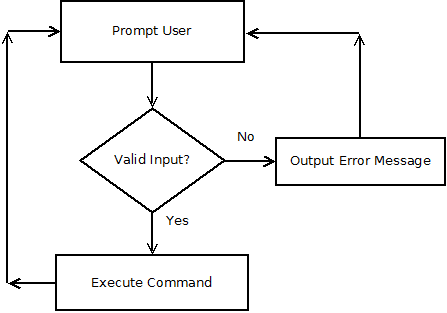
\includegraphics[width=0.7\linewidth]{monitor.png}
			\caption{Structure of Monitor Program}
			\label{fig:monitor}
		\end{figure}
		
		\subsection{Command Interpreter}
			\subsubsection{Algorithm and Flowchart}
			The algorithm for the command interpreter uses simple string matching to determine if input is correct. The algorithm begins by outputting the message \texttt{MONITOR441>} and accepting input from the user. It then checks for the ASCII value \$48 which corresponds to the letter H. This is to check for either the \texttt{HELP} command or \texttt{HXDC} command. If an H was not entered, it then checks for the ASCII value \$4D which corresponds to a memory command. If this fails, then it checks for ASCII value \$47, corresponding to the \texttt{GO} command. If this fails, the ASCII value \$44 is tested, corresponding to the \texttt{DF} command. If this fails, it checks for \$42, which signifies a \texttt{BLCK} command. If this fails, \$53 is tested for the \texttt{SORTW} command. If this fails, \$45 is tested for the \texttt{ECHO} command. If this fails \$2E is checked for the modify register command. If all of these checks fail, the user has entered incorrect input and an error message is displayed. If any of these checks succeed, the command line interpreter jumps to the respective command's helper interpreter function. These subroutines check for each character of the user input in order to verify the command the user entered was correct. These helper functions also serve to differentiate commands that start with the same character. The flowchart for this process is shown in Figure \ref{fig:commandint}.
			
			\begin{figure}[H]
				\centering
				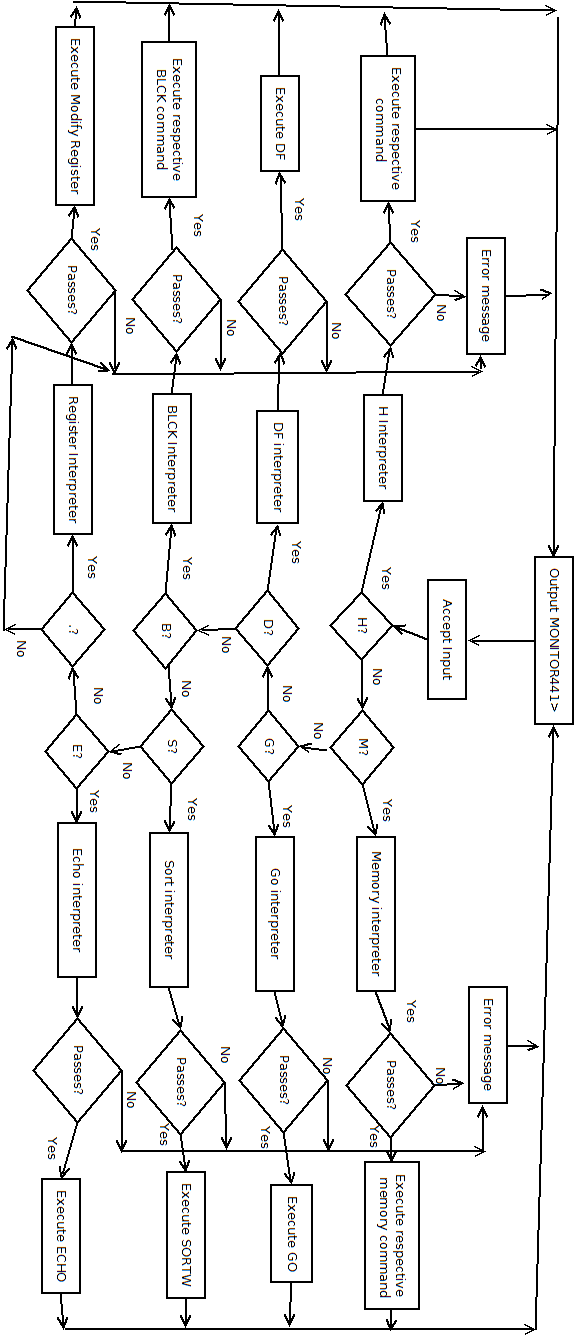
\includegraphics[width=.55\linewidth]{commandint}
				\caption{Flowchart for Command Line Interpreter}
				\label{fig:commandint}
			\end{figure}
			
			\subsubsection{Assembly Code}
			\lstinputlisting[firstline=154,lastline=411,firstnumber=154]{Project.X68}
			
			\subsection{Debugger Commands}
			\subsubsection{Help}
			\paragraph{Algorithm and Flowchart}~\\
			Help is a simple command that prints out a series of strings that display the available commands, their syntax, and a short description of each command. The syntax to invoke this command is \texttt{HELP}. The flowchart for this command is shown in Figure \ref{fig:help}.
			
			\begin{figure}[H]
				\centering
				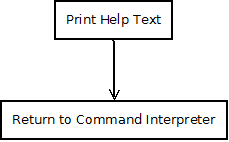
\includegraphics[width=0.4\linewidth]{help}
				\caption{Flowchart for Help}
				\label{fig:help}
			\end{figure}
			
			\paragraph{Assembly Code}~\\
			\lstinputlisting[firstnumber=796,firstline=796,lastline=982]{Project.X68}
			\subsubsection{Memory Display}
			\paragraph{Algorithm and Flowchart}~\\
			Memory display is an extremely useful tool to look at blocks of memory. The syntax to call this function is \texttt{MDSP <address1> <address2}, where \texttt{<address1>} is the starting address and \texttt{<address2>} is the ending address of the memory contents to be shown. This command also displays the block of memory from \texttt{<address1>} to \texttt{<address2 +16bytes>}. The flowchart for this command is shown in Figure \ref{fig:memdsp}.
				
			\begin{figure}[H]
				\centering
				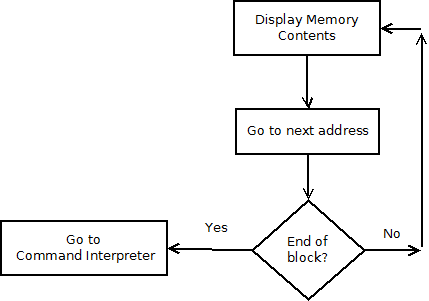
\includegraphics[width=.7\linewidth]{memdsp}
				\caption{Flowchart for Memory Display}
				\label{fig:memdsp}
			\end{figure}
			
			\paragraph{Assembly Code}~\\
			\lstinputlisting[firstnumber=1014,firstline=1014,lastline=1072]{Project.X68}
			
			\subsubsection{HXDEC}
			\paragraph{Algorithm and Flowchart}~\\
			
			\paragraph{Assembly Code}~\\
			\lstinputlisting[firstnumber=1076,firstline=1076,lastline=1135]{Project.X68}
			
			\subsubsection{SORTW}
			\paragraph{Algorithm and Flowchart}~\\
			dfg
			\paragraph{Assembly Code}~\\
			\lstinputlisting[firstnumber=1139,firstline=1139,lastline=1235]{Project.X68}
			
			\subsubsection{Memory Modify}
			\paragraph{Algorithm and Flowchart}~\\
			\paragraph{Assembly Code}~\\
			\lstinputlisting[firstnumber=1239,firstline=1239,lastline=1517]{Project.X68}
			
			\subsubsection{Memory Set}
			\paragraph{Algorithm and Flowchart}~\\
			\paragraph{Assembly Code}~\\
			\lstinputlisting[firstnumber=985,firstline=985,lastline=1012]{Project.X68}
			
			\subsubsection{Block Fill}
			\paragraph{Algorithm and Flowchart}~\\
			\paragraph{Assembly Code}~\\
			\lstinputlisting[firstnumber=1522,firstline=1522,lastline=1574]{Project.X68}
			
			\subsubsection{Block Move}
			\paragraph{Algorithm and Flowchart}~\\
			\paragraph{Assembly Code}~\\				\lstinputlisting[firstnumber=1577,firstline=1577,lastline=1652]{Project.X68}
			
			\subsubsection{Block Test}
			\paragraph{Algorithm and Flowchart}~\\
			\paragraph{Assembly Code}~\\				\lstinputlisting[firstnumber=1656,firstline=1656,lastline=1765]{Project.X68}
			
			\subsubsection{Block Search}
			\paragraph{Algorithm and Flowchart}~\\
			\paragraph{Assembly Code}~\\				\lstinputlisting[firstnumber=1769,firstline=1769,lastline=1887]{Project.X68}
			
			\subsubsection{Go}
			\paragraph{Algorithm and Flowchart}~\\
			\paragraph{Assembly Code}~\\				\lstinputlisting[firstnumber=1891,firstline=1891,lastline=1905]{Project.X68}
			
			\subsubsection{Display Formatted Registers}
			\paragraph{Algorithm and Flowchart}~\\
			\paragraph{Assembly Code}~\\				\lstinputlisting[firstnumber=1909,firstline=1909,lastline=2312]{Project.X68}
			
			\subsubsection{Modify Register}
			\paragraph{Algorithm and Flowchart}~\\
			\paragraph{Assembly Code}~\\				\lstinputlisting[firstnumber=413,firstline=413,lastline=793]{Project.X68}
			
			\subsubsection{Echo}
			\paragraph{Algorithm and Flowchart}~\\
			\paragraph{Assembly Code}~\\				\lstinputlisting[firstnumber=398,firstline=398,lastline=411]{Project.X68}
			
			\subsection{Subroutines}
			
			\subsubsection{Hexadecimal to ASCII}
			\paragraph{Algorithm}~\\
			\paragraph{Assembly Code}~\\				\lstinputlisting[firstnumber=2516,firstline=2516,lastline=2554]{Project.X68}
			
			\subsubsection{ASCII to Hexadecimal}
			\paragraph{Algorithm}~\\
			\paragraph{Assembly Code}~\\				\lstinputlisting[firstnumber=2487,firstline=2487,lastline=2513]{Project.X68}
			
			\subsubsection{BCD to Hexadecimal}
			\paragraph{Algorithm}~\\
			\paragraph{Assembly Code}~\\				\lstinputlisting[firstnumber=2475,firstline=2475,lastline=2485]{Project.X68}
			
			\subsubsection{ASCII to BCD}
			\paragraph{Algorithm}~\\
			\paragraph{Assembly Code}~\\				\lstinputlisting[firstnumber=2464,firstline=2464,lastline=2472]{Project.X68}
			
			\subsection{Exception Handlers}
			The Monitor441 program uses custom exception handlers. They are loaded using the source code:
			\lstinputlisting[firstnumber=134,firstline=134,lastline=151]{Project.X68}
			\subsubsection{Bus Error Exception}
			\paragraph{Algorithm and Flowchart}~\\
			\paragraph{Assembly Code}~\\				\lstinputlisting[firstnumber=2320,firstline=2320,lastline=2357]{Project.X68}
			
			\subsubsection{Address Error Exception}
			\paragraph{Algorithm and Flowchart}~\\
			\paragraph{Assembly Code}~\\				\lstinputlisting[firstnumber=2359,firstline=2359,lastline=2396]{Project.X68}
			
			\subsubsection{Illegal Instruction Error Exception}
			\paragraph{Algorithm and Flowchart}~\\
			\paragraph{Assembly Code}~\\				\lstinputlisting[firstnumber=2398,firstline=2398,lastline=2405]{Project.X68}
			
			\subsubsection{Privilege Violation Error Exception}
			\paragraph{Algorithm and Flowchart}~\\
			\paragraph{Assembly Code}~\\				\lstinputlisting[firstnumber=2407,firstline=2407,lastline=2414]{Project.X68}
			
			\subsubsection{Divide by Zero Error Exception}
			\paragraph{Algorithm and Flowchart}~\\
			\paragraph{Assembly Code}~\\				\lstinputlisting[firstnumber=2416,firstline=2416,lastline=2423]{Project.X68}
			
			\subsubsection{A Line Emulator Error Exception}
			\paragraph{Algorithm and Flowchart}~\\
			\paragraph{Assembly Code}~\\				\lstinputlisting[firstnumber=2425,firstline=2425,lastline=2432]{Project.X68}
			
			\subsubsection{F Line Emulator Error Exception}
			\paragraph{Algorithm and Flowchart}~\\
			\paragraph{Assembly Code}~\\				\lstinputlisting[firstnumber=2434,firstline=2434,lastline=2441]{Project.X68}
			
			\subsubsection{Check Instruction Error Exception}
			\paragraph{Algorithm and Flowchart}~\\
			\paragraph{Assembly Code}~\\				\lstinputlisting[firstnumber=2443,firstline=2443,lastline=2450]{Project.X68}
			
			\subsection{User Instruction Manual Exception Handlers}
			\paragraph{Algorithm and Flowchart}~\\
			\paragraph{Assembly Code}~\\
			
			\section{Discussion}
			
			\section{Feature Suggestions}
			
			\section{Conclusion}
			
			\begin{thebibliography}{1}
				\bibitem{tst} test
			\end{thebibliography}
\end{document}